% Copyright 2009 by Joyan <joyanlj@gmail.com>.
% Last Modified Feb. 20, 2009
%
% In principle, this file can be redistributed and/or modified under
% the terms of the GNU Public License, version 2.
%
% However, this file is supposed to be a template to be modified for
% your own needs. For this reason, if you use this file as a template
% and not specifically distribute it as part of a another
% package/program, I grant the extra permission to freely copy and
% modify this file as you see fit and even to delete this copyright
% notice.

\documentclass[a4paper,dvipdfm]{article}
\usepackage[BoldFont,SlantFont,CJKnumber]{xeCJK}%配合xetex >0.997解决
                                %中英文显示问题
\usepackage{indentfirst}%用于首行缩进
%\usepackage[width=500pt]{geometry}%用于设置页面大小
\usepackage[dvipdfm]{graphicx}
\usepackage[usenames,dvipsnames]{color}
\usepackage{xcolor}
%\usepackage{threeparttable}%用于表格内注释
%\usepackage[centerlast]{caption2} %浮动图形和表格标题样式
%\usepackage[rightcaption]{sidecap}%轻松的得到标题在一边的浮动图形或表格
%\usepackage{colortbl}%彩色表格
%\usepackage{multirow}%排版表格里的跨行文本数据和对齐方式
%\usepackage{textcomp}%常见数理单位和货币符号
%\usepackage[section]{placeins}%立即处理浮动体,section选项要求浮动体在它们所在的章节中排出
\usepackage{subfigure} %%图形或表格并排排列

% \usepackage{fancyhdr}%设置页眉页脚
% \fancypagestyle{plain}{%
%   \fancyhf{}              
%   \fancyhead[R]{\thepage}
%   \fancyhead[L]{00648333}
% }
% \fancyhead[R]{\thepage}
% \fancyhead[L]{00648333}
% \pagestyle{fancy}

% \usepackage{setspace}%设置行距
% \doublespacing%双倍行距

% \usepackage[dvipdfm,a4paper,CJKbookmarks,bookmarks=true,bookmarksopen=true]{hyperref}%很强大的一个东西
% \hypersetup{
%     pdftitle={},
%     pdfauthor={Wen Zhang},
%     pdfkeywords={},
%     bookmarksnumbered,
%     pagebackref=true,
%     breaklinks=true,
% %    pdfview=FitH,       % Or try pdfstartview={FitV}, This lead to uncorrect bookmarks
%     urlcolor=cyan,
%     colorlinks=true,
%     citecolor=magenta,          %citeref's color
%     linkcolor=magenta,
%         }



\DeclareGraphicsExtensions{.eps,.ps,.eps.gz,.ps.gz,.eps.Z,.EPS,.pdf,.PDF,.jpg}%声明图片后缀

\newcommand{\chuhao}{\fontsize{42pt}{\baselineskip}\selectfont}
\newcommand{\xiaochuhao}{\fontsize{36pt}{\baselineskip}\selectfont}
\newcommand{\yihao}{\fontsize{28pt}{\baselineskip}\selectfont}
\newcommand{\erhao}{\fontsize{21pt}{\baselineskip}\selectfont}
\newcommand{\xiaoerhao}{\fontsize{18pt}{\baselineskip}\selectfont}
\newcommand{\sanhao}{\fontsize{15.75pt}{\baselineskip}\selectfont}
\newcommand{\sihao}{\fontsize{14pt}{\baselineskip}\selectfont}
\newcommand{\xiaosihao}{\fontsize{12pt}{1.3\baselineskip}\selectfont}
\newcommand{\wuhao}{\fontsize{10.5pt}{1.3\baselineskip}\selectfont}
\newcommand{\xiaowuhao}{\fontsize{9pt}{\baselineskip}\selectfont}
\newcommand{\liuhao}{\fontsize{7.875pt}{\baselineskip}\selectfont}
\newcommand{\qihao}{\fontsize{5.25pt}{\baselineskip}\selectfont}

\defaultfontfeatures{Mapping=tex-text}
\setmainfont{Droid Sans}% 设置缺省英文字体
\setCJKmainfont[BoldFont=SimHei,ItalicFont=KaiTi_GB2312]{SimSun}% 设置缺省中文字体

\renewcommand\refname{参考文献}

\newcommand{\upcite}[1]{\textsuperscript{\cite{#1}}} %自定义命令\upcite, 使参考文献引用以上标出现

\graphicspath{{figures/}}

\renewcommand\contentsname{目录}
\renewcommand\listfigurename{插图索引}
\renewcommand\listtablename{表格索引}
\newcommand\listequationname{公式索引}
\newcommand\equationname{公式}
\renewcommand\refname{参考文献}
\renewcommand\indexname{索引}
\renewcommand\figurename{图}
\renewcommand\tablename{表}
% \newcommand\CJKprechaptername{第}
% \newcommand\CJKchaptername{章}
% \newcommand\CJKthechapter{\@arabic\c@chapter}
% \renewcommand\chaptername{\CJKprechaptername~\CJKthechapter~\CJKchaptername}
\renewcommand\appendixname{附录}

\makeatletter
\newenvironment{tablehere}
  {\def\@captype{table}}
  {}

\newenvironment{figurehere}
  {\def\@captype{figure}}
  {}
\makeatother



\begin{document}

%%%%%%%%%%%%%%%%%%%%%%%%%%% 正文开始 %%%%%%%%%%%%%%%%%%%%%%%%%%%%%%

\wuhao

\title{穿越时空的门}
\author{陈志杰 \\ zhijiechn@gmail.com}
\date{May. 2009}

\maketitle

\begin{abstract}
  本文以古罗马从奥古斯都建国到君主制的罗马帝国,再到罗马帝国分裂、东西
  罗马帝国的衰落的这段千年罗马史为线索,带领读者一起走进古罗马凯旋门的
  世界,一同欣赏这随着罗马帝国的兴衰而兴衰的凯旋门建筑艺术和变迁。
\end{abstract}
\textbf{关键字:}古罗马,拱门,凯旋门

\tableofcontents

\clearpage

\listoffigures

\clearpage

\section{绪论——门}

门,是人们在日常生活中再熟悉不过的一类建筑,一般来说,只要存在两个世界
的分隔,只要不是完全隔绝,总会有门的存在,门的存在,连接了两个不同世界。
基于门的以上用途,人们给门赋予了许多象征的意义,如门本身预示着一个新的
环境即将到来,代表新的开始和新的纪元;从门內经过,代表着一个世界或者事
件的终结,也预示着新的世界或者事件的开始;不仅如此,从门内经过,还被世
界各地的人们用来进行各种仪式,如中国古代的皇帝,每次出城围猎,往往在城
门周围聚集着各种各样的人,围猎的队伍也是在经过城门的时候走的最``雄赳赳
气昂昂'';其他的各种出发仪式和归来仪式也大都是围绕着门来进行的。这篇文
章所要介绍给大家的,也是一种门,这种门雄伟庄严,这种门鬼斧神工,这种门
展示了人类的祖先对于美和艺术的求索,这种门记录了一个伟大而灿烂的文明的
兴衰,它们就是分布在现今地中海附近的,古罗马凯旋门。下面,就让我们透过
这扇门,一起穿越时空,领略古罗马文明独有的艺术魅力,聆听这一座座凯旋门
向我们诉说的千年一前的故事。

\section{古罗马凯旋式}

说到古罗马凯旋门,就不得不先提一下古罗马的凯旋式。罗马凯旋式(The Roman
triumph, or triumphus),是古罗马授予取得重大军事成果,特别是那些获得打
赢了一整场战争的军事将领的庆祝仪式。对于统治罗马的贵族而言,凯旋式是最
大且最受欢迎的荣耀。获得凯旋式的将领被称为凯旋者(或凯旋英雄,拉丁文(后
文用Latin标示):vir triumphalis),并且有权在其余生中保留使用这一称号的
权利。在他死后,每当其家族举行葬礼时,都会雇佣一名演员戴上他的死亡面
具(Latin:imago),穿上其在凯旋式上穿着过的紫色绣金的刺绣托加相同的托
加,以彰显其生前的成就。关于这项仪式的起源,目前史学界还有许多争议,本
文也暂不讨论,但是其目的则是比较明确的:用来纪念某个军事将领及其军队在
重要战争中的胜利,也同时纪念某一个战争的结束。这种纪念仪式的兴起早于罗
马建国,但在罗马帝国时期达到顶峰。凯旋式的最主要环节是从在瑟维尔
墙(Servian Walls)之外的战神广场(Campus Martius)上一直到卡皮托林
山(Capitoline Hill )上的神庙(Temple of Iuppiter Capitolinus)中的一
长段庄严隆重的环节,由于本文主要讨论的内容古罗马凯旋门,因而这一部分在
此不展开详述,详见。

在凯旋式上,通常还有新的纪念物被树立以纪念着这场凯旋式,其中最壮观
的,就是各种各样的凯旋门。凯旋门与一般的城门不同,通常为横跨在一条道路
之上的独立性建筑,在凯旋门下经过,也往往更多是一种仪式和象征。

凯旋门起源于凯旋式,但并不局限于此,在后来的发展中,凯旋门的意义和用途
被人们扩大,逐渐成为独立的用来纪念的标志物。

\section{古罗马凯旋门}

\subsection{凯旋门的主要结构}

凯旋门是一个巨大的拱形建筑,典型的古罗马凯旋门是独立于城墙的,也就是说
它并不具有一般门的那种为分割的区域提供捷径的功能,而更多的是作为一种符
号和纪念引起人们的注意。他以两个柱子以及一个横跨在柱子之上的一个拱形作
为主要骨架,上着各种各样的装饰性花纹和图案。由于凯旋门巨大的结构和对于
稳定性的严格要求,因此主要骨架并不会被精雕细琢,所有的装饰都是以附在主
干上的各种各样栩栩如生的浮雕为主,这些浮雕的主题大多为歌颂胜利,浮雕上
的人物主要有建筑所纪念的对象和事件,军队和战利品,带有翅膀的女性形
象(与后来的宗教作品中的天使比较类似),拱形曲线等。当然,在门的正上
方,一般还会刻有与这次凯旋式或者胜利有关的题词,这也是获取某座凯旋门的
纪念对象和背景的最重要的依据。有些更加精致的凯旋门还会在大门的两侧开两
个小拱门(附属拱门)。

\subsection{凯旋门的历史}

虽然凯旋门早在罗马建国以前就已经出现,但是凯旋门真正发展成熟,直至成为
一件令人惊叹的艺术品,还是要归功于古罗马帝国帝王对于这种纪念形式的热衷。
在初期,凯旋门只是用砖和石头建造的非常简单的临时性纪念建筑,拱上装饰有
奖杯和各种战利品;随着罗马共和国以及罗马帝国国力不断强盛和建造技术的不
断发展,凯旋门的用料和制作工艺页越来越讲究,最终发展成为用上等大理石建
造的,中间承放大型拱石,并被精雕细琢的艺术品。当然,建造凯旋门所用的时
间以及花费的人力物力也随其审美价值和雄伟程度的提高而不断增加。

从罗马建国到公元5世纪,历史上记载的资料显示罗马共建造了三十四座凯旋门式
的拱形建筑,其中大部分现在已经见不到,只有一少部分至今依然存在,下面我
们就以时间和在位执政者的顺序,走进凯旋门的世界,了解和欣赏这一个个人类
智慧和力量的杰作。

需要声明一点的是,以下的时间段划分方法只是根据笔者这几个月来对于凯旋
门/拱门结构的观察和年份的整理,根据其外观和一点点罗马史综合所得,只是
为了在叙述和欣赏凯旋门这一种艺术品的方便而划分,除此之外并无多少学术根
据。

\subsection{古罗马凯旋门的兴起}

这一时期包括奥古斯都建国(朱里亚·克劳狄王朝)以前和建国初期的各种拱拱
门,这个时期的凯旋门并没有统一的制作流程和先进的工艺,大多是用砖石建造
的临时性建筑,因此,很遗憾,它们并没有经受住时间的冲刷,至今已经不存在
与这个世界上,只是从一些史料上能够找到他们的影子,这一时期有记载的凯旋
门主要包括阿卡尔狄乌斯拱门(Latin:Arcus Arcadii Honorii et Theodosii,
405 BC)和非洲西皮翁拱门(Arcus Scipii Africani, 109 BC)

\subsection{奥古斯都大帝时期}

由于奥古斯都大帝在世界各地的赫赫战功,在他在位时期共建造了四座凯旋
门,分别在奥斯塔(Aosta)、法诺(Fano)、罗马和里米尼(Rimini)。

奥斯塔奥古斯都凯旋门(Arch of Augustus in Aosta, 35
BC)\ref{fig:augustusaosta},建于公元前35年,是为了庆祝奥古斯都大帝
在 ``Consul Varro Murena over the Salassi'' 战争中的胜利而建造的,从图
中我们可以看出,此时的建筑仍然是以砖石为主,结构比较简单。

\begin{figure}[hbt!]
  \centering
  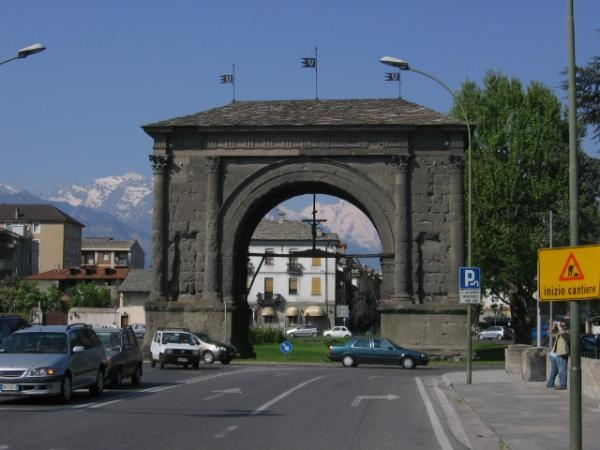
\includegraphics[width=\textwidth]{ArchOfAugustusInAosta}
  \caption{奥斯塔的奥古斯都凯旋门}
  \label{fig:augustusaosta}
\end{figure}

罗马的奥古斯都凯旋门是古罗马广场上的一座凯旋门,完成于公元前29年,庆祝
奥古斯都在亚克兴角战役战胜马克·安东尼和克利奥帕特拉七世。奥古斯都凯旋门
跨越卡斯托尔和波吕克斯神庙和凯撒神庙之间的道路,靠近灶神庙。1546年人们
在这一地点发现了献给奥古斯都的巨大碑刻,因此确定了奥古斯都凯旋门的存在。
奥古斯都凯旋门本身留下的遗迹很少,但是它出现在当时的货币上。它有三个通
道,在罗马首次出现这种样式的拱门,并为塞维鲁凯旋门和后来的君士坦丁凯旋
门所仿效。图\ref{fig:augustusrome1}是当时刻有凯旋门图像的钱
币,图\ref{fig:augustusrome2}是加州大学洛杉矶分校的``Virtual Roman
Forum''项目发布的罗马奥古斯都凯旋门的复原像。从这些资料中我们可以看出这
座凯旋门是三门建筑,支撑柱和上拱比较细,缺乏后来的凯旋门那种庄重威严的
气势,不错由此也可以看出罗马前后期建筑风格从实用主义到越来越花哨的转
变。


\begin{figure}[hbt!]
  \centering
  \subfigure[罗马的奥古斯都凯旋门残片]{
    \label{fig:augustusrome1}
    \includegraphics[width=0.3\textwidth]{Arch_of_August_in_Rome}
  }
  \subfigure[罗马的奥古斯都凯旋门复原图]{
    \label{fig:augustusrome2}
    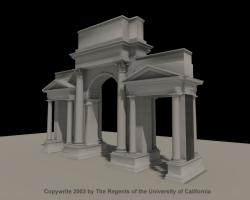
\includegraphics[width=0.6\textwidth]{Arch_of_Augustus_in_Rome_virtual}
  }
  \caption{罗马的奥古斯都凯旋门}
\end{figure}

里米尼的奥古斯都凯旋门是这四个中保存最完整的一个,它建于公元前27年,是
为了纪念奥古斯都建造的,这座凯旋门并不是独立建筑,而是作为城墙的一部分
而建造的,见图\ref{fig:augustusrinimi}。

位于法诺的奥古斯都凯旋门建于公元2年,从图中可以看出这座拱门并不是独立建
筑,同样是由于这一时期的凯旋门的建造并没有特别正式地作为一个单独的项目
和主题受到足够的重视,如图\ref{fig:augustusrifano}。

\begin{figure}[hbt!]
  \centering
  \subfigure[里米尼的奥古斯都凯旋门]{
    \label{fig:augustusrinimi}
    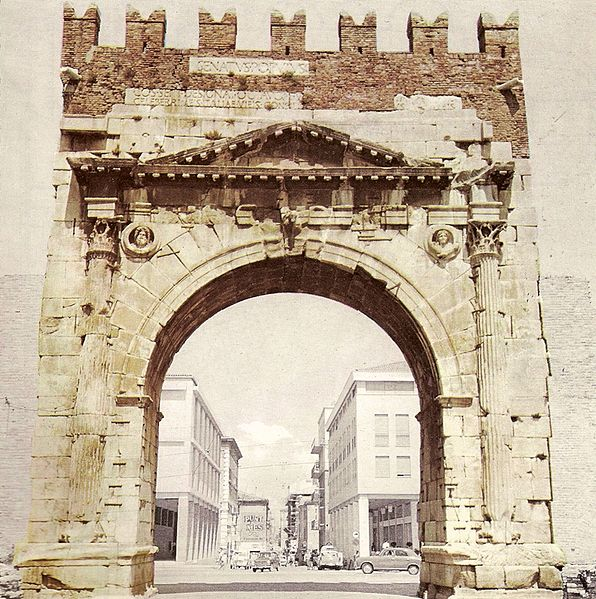
\includegraphics[width=0.45\textwidth]{Arch_og_Augustus_Rimini}
  }
  \subfigure[法诺的奥古斯都凯旋门]{
    \label{fig:augustusrifano}
    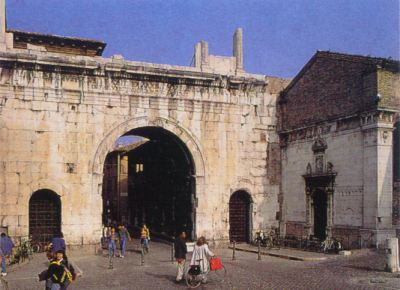
\includegraphics[width=0.45\textwidth]{ArchOfAugustusInFano}
  }
  \caption{奥古斯都凯旋门}
\end{figure}

\clearpage

\subsection{石结构的凯旋门的兴起}

随着古罗马建造技术的不断发展,建造凯旋门的材料逐渐由原来的砖结构转变成
了更加坚固的石结构,这一时期的凯旋门的特点是:

\begin{itemize}
\item 比起以前的凯旋门,规模和坚固程度有了一定程度的提升;
\item 门上的装饰性的结构开始增多,出现了小规模的浮雕;
\item 但是装饰的数量有限,门的主体骨架仍然占用料的主要部分;
\item 门的独立性有了一定程度的提升,但是仍然主要是与其他的建筑配合(特
  别是与桥),作为其他建筑的装饰。
\end{itemize}

这一时期有记载的凯旋门主要有庞特桥上的凯旋门(Arch on Pont Flavien, 12
BC)、德鲁苏斯凯旋门(Arch of Drusus, 三座,分别建于 9 BC, 19 AD 和23
AD)、兰图鲁斯凯旋门(Latin:Arcus Lentuli et Crispini, 2 AD)和多拉贝拉
凯旋门(Latin: Arcus Dolabellae et Silani, 10 AD)。

建于公元前9年的德鲁苏斯拱门,其样子更加像是古罗马初期的拱门的样
式(如图\ref{fig:drusus9bc}),它连同建于公元23年建造的德鲁苏斯拱门(如
图\ref{fig:drusus23bc})都是比较简单的小型拱门,而在公元18-19年,为纪
念德鲁苏斯-日耳曼尼库斯(Drusus Germanicus,因而这个拱门页常被称为是日
耳曼尼库斯拱门)而建造的拱门(如图\ref{fig:germanicus}),连同上面提到
的庞特(Pont Flavien)桥上的凯旋门(如图\ref{fig:pont}),则相对来说要
雄伟的多,至少这两座拱门已经是方方正正,有了后来的凯旋门的样子,从图中
可以看出,拱顶开始有了一圈记述功绩的浮雕。

\begin{figure}[hbt!]
  \centering
  \subfigure[9 BC]{
    \label{fig:drusus9bc}
    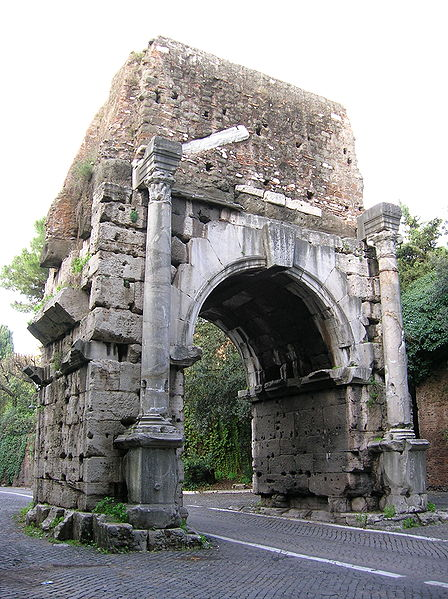
\includegraphics[width=0.45\textwidth]{Arch_of_drusus_9_bc}
  }
  \subfigure[23 AD]{
    \label{fig:drusus23bc}
    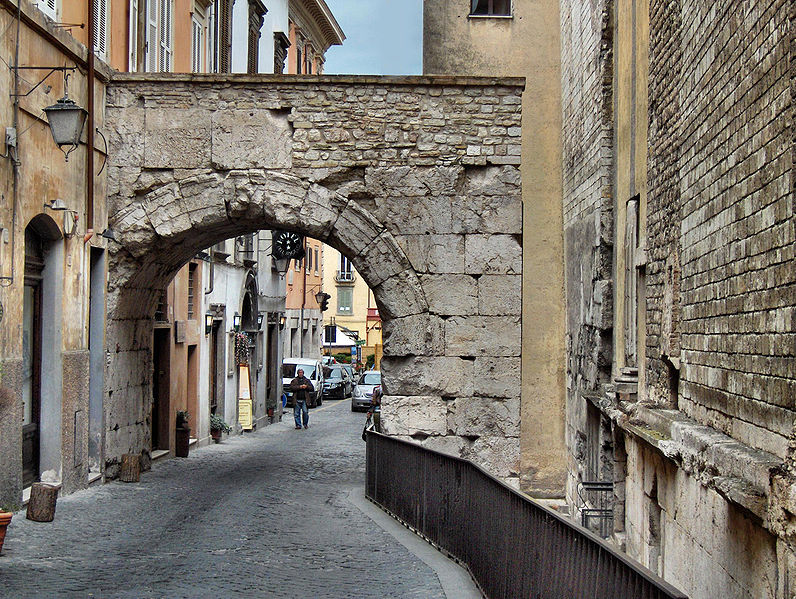
\includegraphics[width=0.45\textwidth]{Arch_of_Drusus_23}
  }
  \caption{德鲁苏斯拱门}
\end{figure}

\begin{figure}[hbt!]
  \centering
  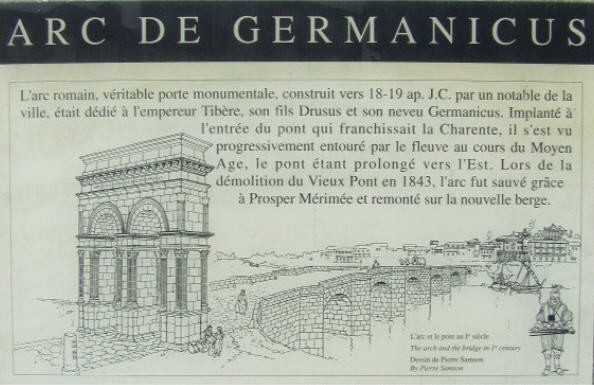
\includegraphics[width=\textwidth]{ArchOfDrusus_of_Germanicus}
  \caption{日耳曼尼库斯拱门}
  \label{fig:germanicus}
\end{figure}

\begin{figure}[hbt!]
  \centering
  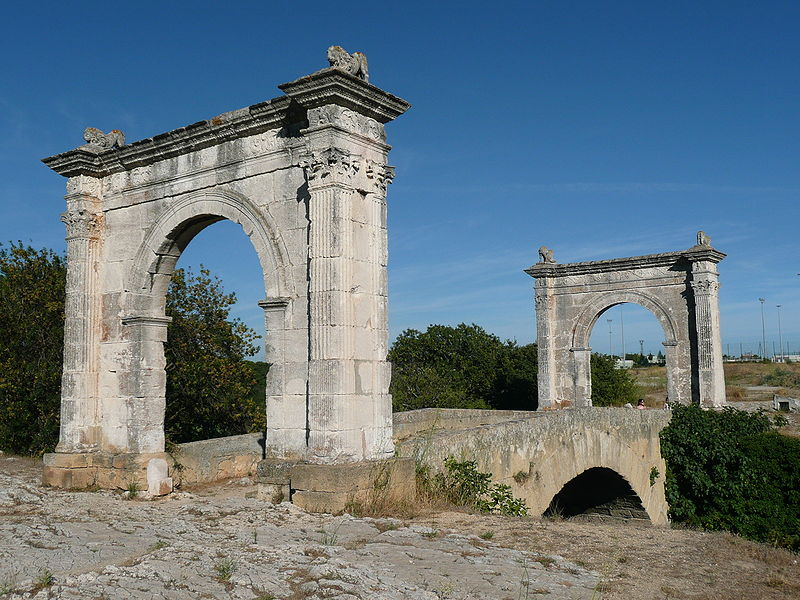
\includegraphics[width=\textwidth]{PontFlavien}
  \caption{庞特桥上的凯旋门}
  \label{fig:pont}
\end{figure}

\clearpage

\subsection{古罗马凯旋门走向鼎盛}

这段时期,古罗马结束了四帝內乱,罗马的政治逐渐稳定下来,社会开始回到正
轨,国力愈加强盛。在这一时期,凯旋门建造技术高度发展,各种样式和浮雕层出
不穷,由于古罗马帝国国立的逐渐强盛,以及劳动力和物产的逐渐丰富,出现了
用名贵的大理石建造的凯旋门,不仅如此,作为凯旋式中越来越重要的一部
分,凯旋门的纪念意义越来越受到人们特别是贵族的青睐,于是,凯旋门作为一
种单独的艺术建筑和象征符号,逐渐摒弃了原来与城墙、桥梁一起的功能性,而
变成了一种纯粹的独立的建筑存在起来。

这段时期,可以继续细分为前期、中期和后期三个阶段:

\subsubsection{前期:凯旋门的独立和定型}

正如这一节的小标题所暗示的那样,这一时期的凯旋门的主要特征是:

\begin{itemize}
\item 凯旋门作为一种重要的纪念和象征,逐渐从整体建筑中独立出来,单独作
  为一种独立的建筑艺术形式。
\item 凯旋门的结构逐渐成熟,样式逐渐固定下来,成为后来的凯旋门效仿的对
  象。
\item 凯旋门的装饰性元素逐渐增多,特别是记叙性和歌颂性的浮雕的出现和增
  多,成为欣赏凯旋门的一个重要方面,也为后来的史学研究提供了大量史料。
\end{itemize}

这一时期从朱里亚·克劳狄王朝末期,横跨四帝内乱期和弗拉维王朝,一直到五贤
帝前期,有记载的凯旋门主要有:奥朗日凯旋门(Triumphal Arch of Orange,
27 AD)、克劳迪乌斯凯旋门(Arch of Claudius, 46-51 AD)、提图斯凯旋
门(Arch of Titus,81 AD)、位于意大利安科纳、贝那芬托、西班牙梅里达的三
座图拉真凯旋门(Arches of Trajan,114)、和哈德良凯旋门(Arch of
Hadrian,131-132 AD)。


\textbf{奥郎日凯旋门}

奥郎日凯旋门(见图\ref{fig:orange})位于今法国奥郎日,关于其始建时
间,其实目前仍然是一个争论的话题,比较令人信服的一个说法是最初是为了纪
念发生于公元前58至52年的高卢战争以及奥古斯都第二军团,后来提贝里乌
斯(Tiberius)皇帝为了纪念发生在莱茵兰(Rhineland)的是日耳曼尼库斯对抗
日耳曼军队的胜利重建了它,从图中我们可以看到,奥郎日凯旋门已经对拱上的
装饰物和浮雕进行了精雕细琢的强调,拱上方的部分几乎占整个门的一半,上方
刻有海战的场景、战利品以及罗马人与高卢和日耳曼人对抗的其他场景。

\begin{figure}[hbt!]
  \centering
  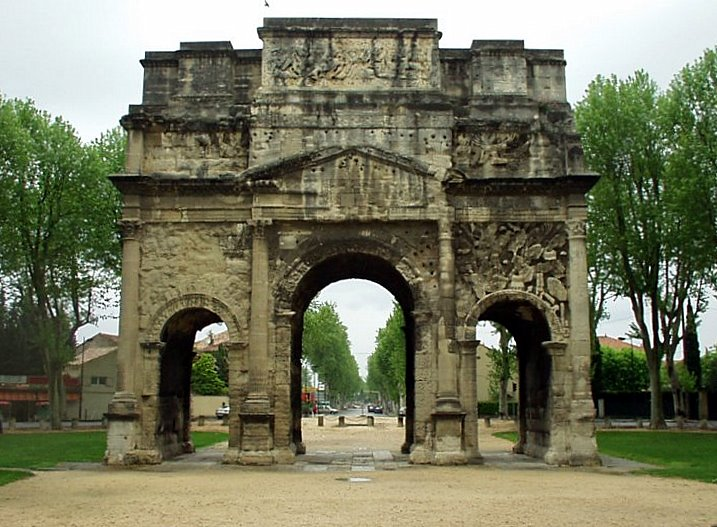
\includegraphics[width=\textwidth]{Arch_of_Orange}
  \caption{奥郎日凯旋门}
  \label{fig:orange}
\end{figure}

整个凯旋门开有三个通道,中间一个较大的,两边一边一个较小的,整个凯旋门
由四列长柱支撑。奥郎日凯旋门是现存最早的用这种结构建造的凯旋门,后来的
塞维勒斯凯旋门(Arch of Septimius Severus)以及著名的君士坦丁凯旋门都
是仿照这种结构建造的。

\textbf{克劳迪乌斯凯旋门}

克劳迪乌斯凯旋门是为了纪念克劳迪乌斯成功入侵不列颠而建造的,现在已经被
毁,仅存一些门上的题词和装饰,保存在卡比托里山博物馆(Capitoline
Museum)。

\textbf{提图斯凯旋门}

提图斯凯旋门(图\ref{fig:titus})是意大利罗马市古罗马广场东南圣道上的一
座大理石单拱凯旋门,由图密善皇帝兴建于兄长提图斯去世后不久,纪念在公
元70年征服和摧毁耶路撒冷,终止66年开始的犹太人大起义。提图斯凯旋门建于
公园81年,是这一时期凯旋门中最具艺术魅力的一个。凯旋门几乎各处都刻有精
美的浮雕作品,尤其是拱门内壁上,拥有现存唯一的对耶路撒冷圣殿器物的描
绘,上面清楚描绘了灯台和小号,可能还有陈设饼桌
子(如图\ref{fig:titus1})。通道的顶部描绘了以被神化的提图斯为中心的方
格浮雕,如图\ref{fig:titus2}。门的正上方使用大写罗马字母提写的题词,写
着``参议院和罗马人民(将此献给)的神圣的提图斯奥古斯都,神圣的维斯帕先
之子''。

\begin{figure}[hbt!]
  \centering
  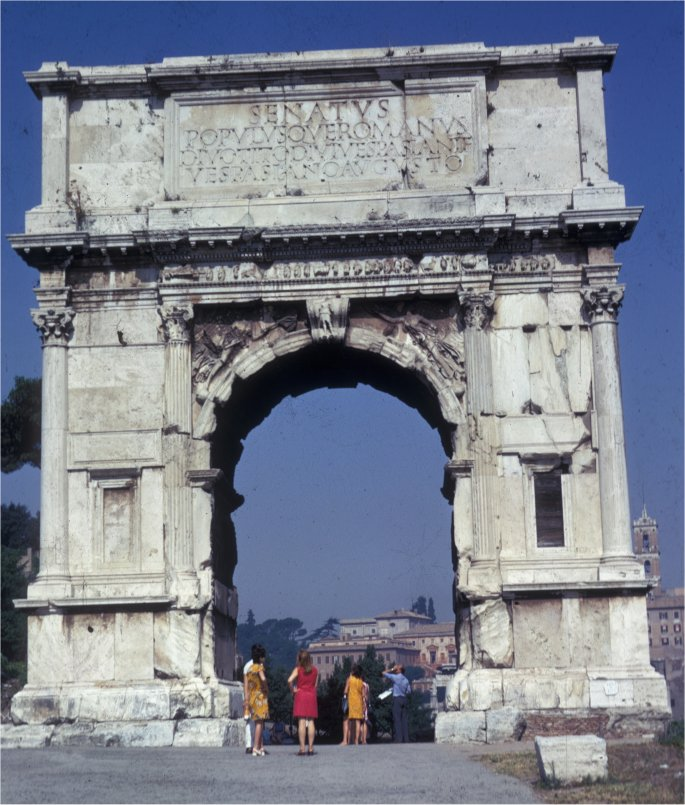
\includegraphics[width=\textwidth]{Arc_de_titus_frontal}
  \caption{提图斯凯旋门}
  \label{fig:titus}
\end{figure}


\begin{figure}[hbt!]
  \centering
  \subfigure[细节一]{
    \label{fig:titus1}
    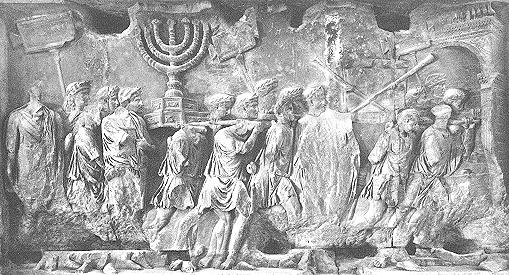
\includegraphics[width=0.45\textwidth]{Arch_of_titus_detail}
  }
  \subfigure[细节二]{
    \label{fig:titus2}
    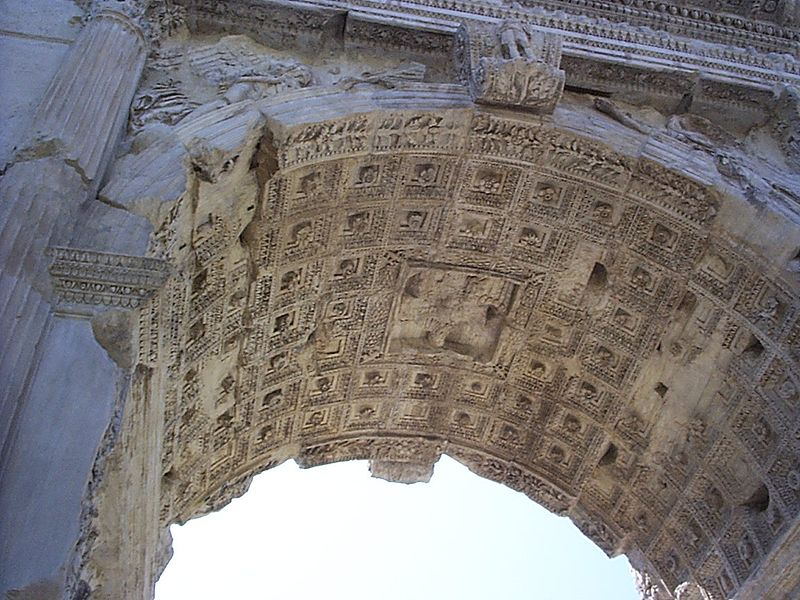
\includegraphics[width=0.45\textwidth]{Arch_of_Titus_TopDetail}
  }
  \caption{提图斯凯旋门}
\end{figure}



提图斯凯旋门的单拱结构和方形的样式,被后来的许多凯旋门所模仿,如法国的
巴黎凯旋门。

\clearpage

\subsubsection{中期:罗马帝国最盛时期的标志}

这个时期从塞维鲁王朝开始,经过3世纪危机,一直到君士坦丁王朝,由于罗马帝
国的国力在此阶段逐渐达到了顶峰,各种凯旋门遍地开花。这个时期有记载的凯
旋门包括:塞维勒斯凯旋门(Arch of Septimius Severus, 203 AD)、加列奴拱
门(Arch of Gallienus 262 AD)、伽列里乌斯凯旋门(Arch of Galerius
298-303 CE)以及君士坦丁凯旋门(Arch of Constantine 315 AD)等等。

\textbf{塞维勒斯凯旋门(或称塞维鲁凯旋门)}

塞维鲁凯旋门(Arch of Septimius Severus)是古罗马广场西北端的一座白色大理
石建筑,建于公元203年,以庆祝塞普蒂米乌斯·塞维鲁皇帝和他的两个儿子卡拉
卡拉和塞普提米乌斯·盖塔在194/195年和197-199年两次战胜波斯。

从图\ref{fig:serverus}中可以看到,塞维鲁凯旋门与提图斯拱门有很多相似之
处,特别是拱顶的方形平台和上面的题字,以及拱门内部通道上的浮雕和拱顶的
方形图案。后来的君士坦丁凯旋门也是如此。

\begin{figure}[hbt!]
  \centering
  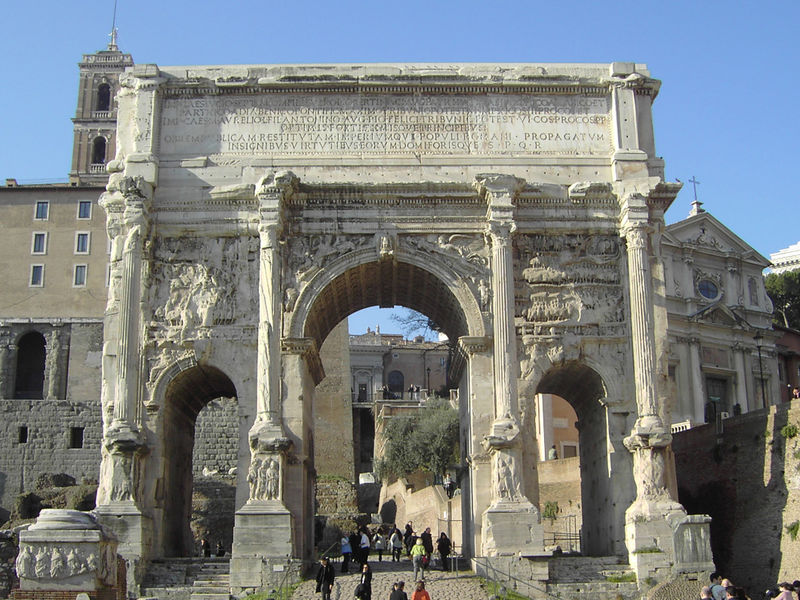
\includegraphics[width=\textwidth]{ArchofSeptimiusSeverus}
  \caption{赛维勒斯凯旋门}
  \label{fig:serverus}
\end{figure}

除了位于古罗马广场的这座,据记载在罗马帝国博亚里昂市场附近还有一个用来
纪念赛维勒斯的凯旋门,建于公元204年,不过现已无从寻找。


\textbf{君士坦丁凯旋门}

最终,我们终于来到了古罗马现存最大最雄伟的凯旋门——君士坦丁凯旋门面
前(如图)。君士坦丁凯旋门建于于公元312年,是为庆祝君士坦丁大帝于公
元312年彻底战胜他的强敌马克森提,并统一帝国而建的。风格上借鉴了在他之前
的提图斯拱门和赛维勒斯凯旋门的设计。

\begin{figure}[hbt!]
  \centering
  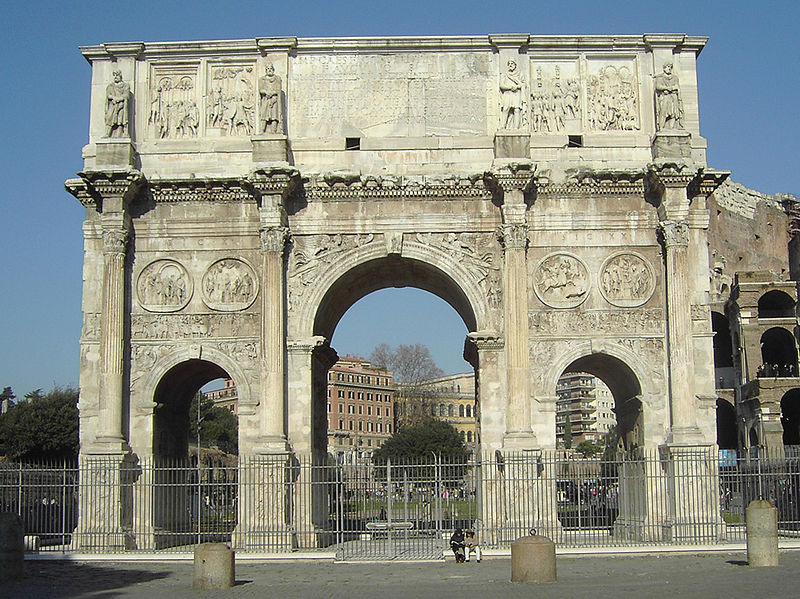
\includegraphics[width=\textwidth]{ConstantineArch}
  \caption{君士坦丁凯旋门}
  \label{fig:contiantine}
\end{figure}

\begin{figure}[hbt!]
  \centering
  \subfigure[细节一]{
    \label{fig:contiantine1}
    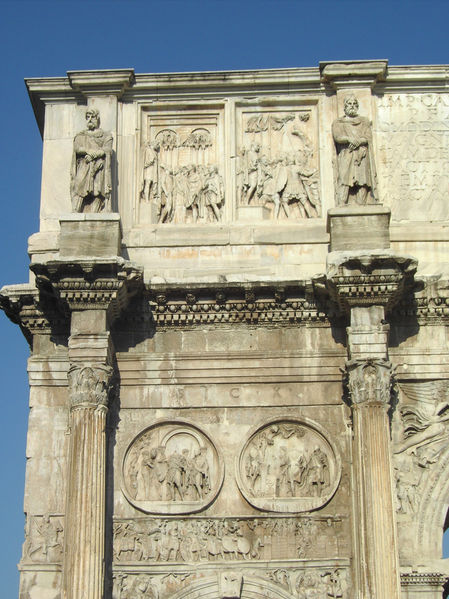
\includegraphics[width=0.45\textwidth]{Arch_of_Constantine_Deatails00}
  }
  \subfigure[细节二]{
    \label{fig:contiantine2}
    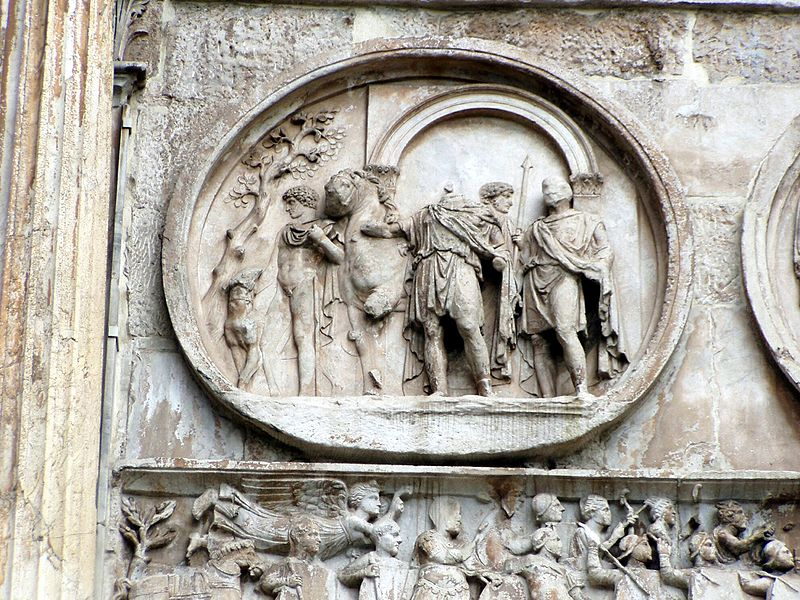
\includegraphics[width=0.45\textwidth]{Arch_of_Constantine_Deatails01}
  }
  \caption{君士坦丁凯旋门}
\end{figure}

\begin{figure}[hbt!]
  \centering
  \subfigure[细节三]{
    \label{fig:contiantine3}
    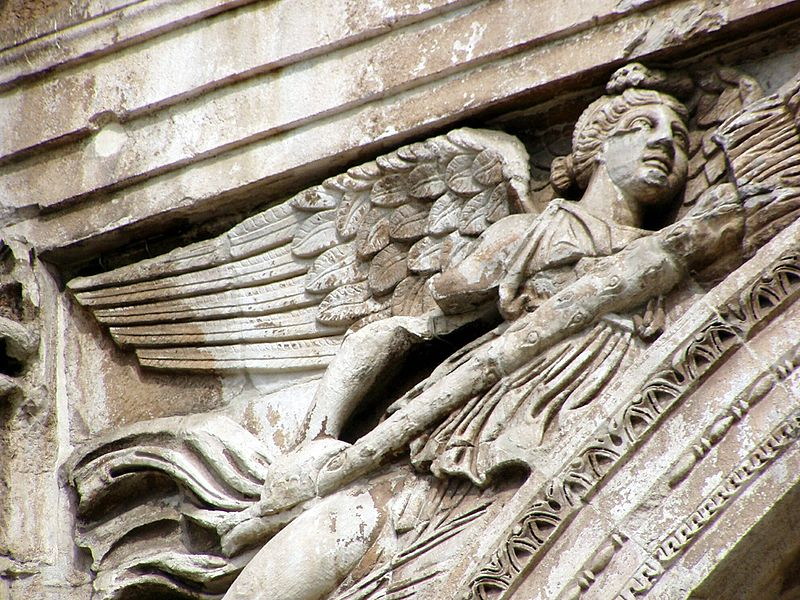
\includegraphics[width=0.45\textwidth]{Arch_of_Constantine_Deatails02}
  }
  \subfigure[细节二]{
    \label{fig:contiantine4}
    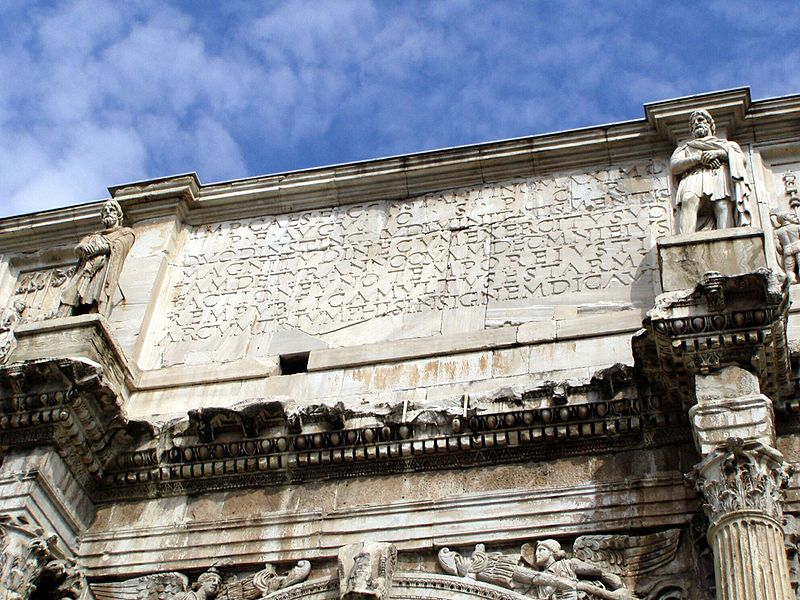
\includegraphics[width=0.45\textwidth]{Arch_of_Constantine_Deatails03}
  }
  \caption{君士坦丁凯旋门}
\end{figure}

\begin{figure}[hbt!]
  \centering
  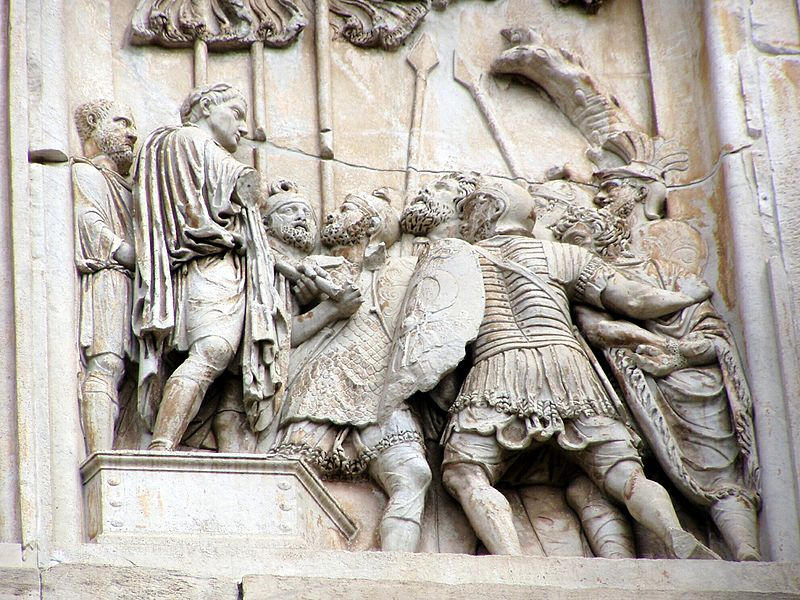
\includegraphics[width=0.8\textwidth]{Arch_of_Constantine_Deatails04}
  \caption{君士坦丁凯旋门细节五}
  \label{fig:contiantine5}
\end{figure}

这是一座三个拱门的凯旋门,高21米,面阔25.7米,进深7.4米。由于它调整了高
与阔的比例,横跨在道路中央,显得形体巨大。凯旋门的里里外外充满了各种浮
雕,表面上看去,巨大的凯旋门和丰富的浮雕虽然气派很大,但缺乏整体观念。
原因是凯旋门的各个部分并非作为一个统一体而创作的,甚至其中的大部分构件
是从过去的一些纪念性建筑,如图拉真广场建筑上的横饰带、哈德良广场上一系
列盾形浮雕以及马克·奥尔略皇帝纪念碑上的八块镶板,拆除过来的。尽管如
此,它仍不失为一座宏伟壮观的凯旋门,尤其是它上面所保存的罗马帝国各个重
要时期的雕刻,是一部生动的罗马雕刻史。

从这座雄伟巨大的建筑中,我们可以看到当时罗马帝国的强盛。然而仔细观察的
话,从各处挪移过来的各种装饰,生硬的拼错在一起,虽然使得这座凯旋门雄伟
气派,但是却丧失了自己的风格,甚至连君士坦丁皇帝的雕像,也是用别人的雕
像换成君士坦丁皇帝的头像。以上种种迹象,似乎也暗示了罗马帝国极盛的浮华
表面下隐藏的各种矛盾和衰落的趋势。

\clearpage

\subsubsection{后期:古罗马帝国和凯旋门的安魂曲}

君士坦丁一世死后,国分为三,君士坦丁二世、君士坦提乌斯二世和君士坦斯一
世各掌其一,从此,罗马帝国走向彻底衰落,长期的混乱和其他民族的统治使凯
旋门的建造几乎被人遗忘,这一时期有记载的凯旋门只有格拉蒂安凯旋
门(Latin: Arcus Gratiani Valentiniani et Theodosii,379-383)和雅努斯
凯旋门(Arch of Janus,405)。


\textbf{雅努斯凯旋门}

雅努斯凯旋门(The Arch of Janus)建于公元405年(一说四世纪早期),是为
了纪念君士坦丁王朝的强盛而建造的,如图\ref{fig:janus},它是现存的唯一一
座四面的拱门\ref{fig:janusl},这座拱门已经没有前面的那些凯旋门的凌人气
势和雄伟姿态,变得矮小朴素,据记载该拱门常被用来拱市场上的商人遮风挡雨
之用。

\begin{figure}[hbt!]
  \centering
  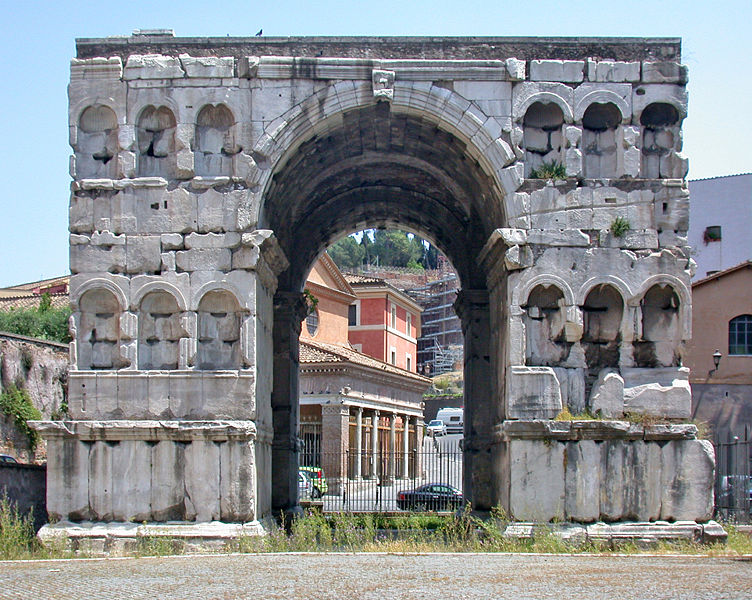
\includegraphics[width=\textwidth]{Arch_of_Janus}
  \caption{雅努斯凯旋门}
  \label{fig:janus}
\end{figure}

\begin{figure}[hbt!]
  \centering
  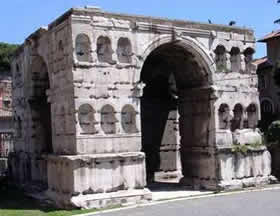
\includegraphics[width=0.5\textwidth]{arch_of_janus_left}
  \caption{雅努斯凯旋门侧面}
  \label{fig:janusl}
\end{figure}

\subsection{后凯旋门时期}

随着罗马帝国的灭亡,使得凯旋门风光不再,虽然偶尔也会有星星点点类似凯旋
门的建筑在世界各地被建造,但比起罗马时期的兴盛,无论在规模上还是数量上
已不可同日而语,直到一千年后的文艺复兴时期。

由于文艺复兴时期人们打出的旗号和当时思潮的影响,古罗马式的凯旋门逐渐又
开始受到人们的欢迎,在十五到十九世纪,国王和皇帝们陆续建造了许多模仿古
罗马凯旋门式的建筑,最早的如意大利那不勒斯的阿拉贡拱门(Aragonese
Arch),1443年由阿丰索五世(Alfonso V)兴建,以及最著名的巴黎凯旋
门(Arc de Triomphe in Paris)。

巴黎凯旋门,即雄狮凯旋门,位于法国巴黎的戴高乐广场中央,是拿破仑为纪
念1805年打败俄奥联军的胜利,于1806年下令修建而成的。拿破仑被推翻后,凯
旋门工程中途辍止。波旁王朝被推翻后又重新复工,直到20年后的1836年终于全
部竣工。


\begin{figure}[hbt!]
  \centering
  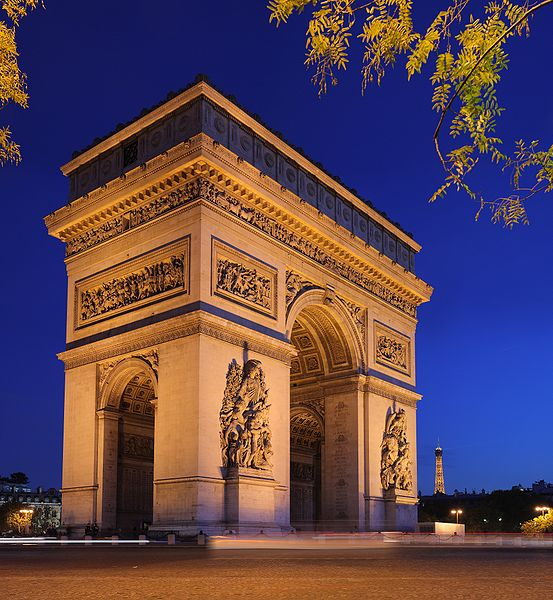
\includegraphics[width=\textwidth]{Arc_de_Triomphe}
  \caption{巴黎凯旋门}
  \label{fig:par}
\end{figure}


巴黎凯旋门高49.54米,宽44.82米,厚22.21米,中心拱门高 36.6米,宽14.6米。
在凯旋门两面的墙面上是四组以战争为题材的大型浮雕:``出征''、``胜利''、
``和平''和``抵抗'',门内刻有跟随拿破仑远征的386名将军和96场胜仗的名字。

在上面的发展过程中,凯旋门这一词所代表的意义已经跟最初有了很大的差别,
凯旋门已经不只是凯旋式的一部分,而是独立出来,作为一种对于重大事件的纪
念形式,广泛应用起来。

\clearpage

\section{总结}

绵延千年的古罗马文明为世界文化、艺术、政治等各个领域带来了丰富的宝藏和
财富。凯旋门,作为古罗马的象征之一,不仅是古罗马文明带给世界的建筑奇
迹,也是古罗马文明从起源到鼎盛再到衰落的忠实记载。每当我无论是在图书馆
捻过一页页画册、还是在网上点击一张张图片,都会对着这些充满神秘的震撼的
感觉的门陷入沉思,仿佛门的另一侧就是长长的罗马历史和人类历史。每次我都
想:当我们在欣赏这些建筑史上的奇迹,为在当时环境下竟然能够完成如此鬼斧
神工的艺术所惊叹的时候,还应该注意到艺术和艺术史所带给我们的,不仅是美
的享受,视觉的盛宴,更是一次对于人类文化和文明的探究和思索,对于人类本
性的一种拷问和展示。

\cite{*}

\appendix{}

\bibliography{bibdb}
\bibliographystyle{unsrt}


\end{document}
%%% Local Variables: 
%%% mode: latex
%%% TeX-master: t
%%% End: 
